\begingroup
\clearpage% Manually insert \clearpage
\let\clearpage\relax% Remove \clearpage functionality
\vspace*{-16pt}% Insert needed vertical retraction
\chapter[THE STANDARD MODEL]{THE STANDARD MODEL}
\endgroup

\begin{alltt}
{\footnotesize \centering
"The effort to understand the universe is one 
of the very few things that lifts human life
a little above the level of farce, and gives 
it some of the grace of tragedy." 
                                  - \emph{Steven Weinberg, 1993}}                               
\end{alltt}


\section{A Model of Leptons}

Back in 1967 Steven Weinberg outlined the foundation of what would become the Standard Model (\gls{sm}) in 
a three paged Physical Review letter titled \emph{A Model of Leptons}. Here he stated "What could be more 
natural than to unite [leptons, photons, and their intermediate bosons] into a a multiplet
of gauge fields?" \cite{weinberg}. This quote could not have been more of an understatement.
The model that was predicted in this letter would later become the most successful theory ever
conceived. The \gls{sm}'s articulate description of the universe predicted particles that
were all later found including the latest particle, the Higgs boson. 
\par
This theoretical formulation was not conceived by Weinberg out of nowhere. It was an inevitable outcome 
from a composition of works. The first came from Yang Chen-Ning and Robert Mills, they provided an explanation
for strong interactions via gauge theory in their 1954 paper \cite{yang-mills}. Then came Chien-Shiung Wu 
demonstrating the non-conservation of parity in the weak interaction in 1957 \cite{wu}.
Sheldon Lee Glashow proposed the bold \boldmath{SU(2) × U(1)} model that showed
the possibility of symmetry between electromagnetic and weak interactions which in turn predicted
the Z boson \cite{Glashow}. 
\par
Steven Weinberg was in close contact with Abdus Salam during the year of 1961.
This led Abdus Salam and his long time collaborator John C. Ward to proposing a very similar model to 
Glashow's \boldmath{SU(2) × U(1)} \cite{Salam}. Though both of these models still required
the masses for the W and Z bosons to be inserted by hand making the model non-renormalizable and thus
non-physical. Lastly, to put all the puzzle pieces together, Peter Higgs came in and 
demonstrated spontaneous symmetry breaking via the Higgs mechanism \cite{Higgs}. 
Three years later in just three pages, Weinberg formulated the first iteration of the \gls{sm} in 1967 \cite{weinberg}.

\section{The Standard Model}
\label{sect:standard_model}

The \gls{sm} of particle physics is one of the most successful theories that has been proposed in 
modern physics. It has predicted elementary and composite particles that scientists are still discovering 
to this day with the latest being the Higgs boson. It has withstood countless experimental checks as global
scientific communities from all around the world have given billions towards this vast area of research. Creating 
one of the largest collaborations in the world with this model at its heart. The \gls{sm} is a model 
of symmetries and how these symmetries break, creating elementary particles. The elementary particles predicted by 
the \gls{sm} can be split into two groups as seen in Figure \ref{fig:sm_fig}. There are the matter particles (purple and green) 
and the force particles (red and yellow). The matter particles can also be called fermions and are split into three 
generations. There are the quarks (up, down, strange, charm, bottom, top) and there 3 leptons 
(electron, muon and the tau lepton) and their corresponding neutrino (electron neutrino, muon neutrino and tau lepton neutrino). 
There are then the force carrying bosons along with the Higgs boson which is responsible for the Higgs mechanism and is discussed
later in this chapter. How these elementary particles interact with one another is described by the force carrying particles. 
These particles are the photon ($\gamma$), gluon, $W$ and $Z$ bosons. Each of these force carrying particles mediate a corresponding force. 
All physical phenomena are interactions of forces which include four types; the electromagnetic force, gravitational force, 
the strong force and the weak force. As the \gls{sm} was in its infancy, it started to reveal the possibility that 
these forces were combined as a single force at one point in time. The current state of the \gls{sm} is unable to
relate the gravitational force to the other three forces, though this problem is well known and decades of careers are 
being put forth to solve this hole. 
\par
Now each force has its own responsibility. The gravitational force is what everyone interacts with everyday
since it's the reason we simply don't float off into space. Gravity is well described on a macro scale through 
the beautiful theory of General Relativity which describes the interactions between macro objects 
such as planets and stars, though this is beyond the scope of this thesis and is well described in the field 
of astrophysics and astronomy. Currently gravity's interaction on the scale of the \gls{sm} is so 
small, it's negligible, and has no relevance in understanding elementary particle interactions (at least to 
our current knowledge). The predicted force carrying particle is called the Graviton and it has eluded 
experiments since its formulation.
The electromagnetic force is used to communicate between charged particles.
This force is magnitudes stronger than the gravitational force and therefore has repercussions dictating
the relationships on all scales. The force carrying particle is called the photon which is a massless boson. This elementary particle is a quantum of the electromagnetic field. 
Meaning, it's the bare minimum particle involved in interactions within this field. 
The strong force is the fundamental interaction that binds elementary particles, creating larger composite particles 
called hadrons. This force is mediated by the boson called a Gluon. Gluons are massless vector bosons and the binding of 
quarks are in accordance with Quantum Chromodynamics (\gls{qcd}). These bosons carry color charge which adds a layer of complexity
and is the reason gluons participate in this interaction. The strong force can also be called the nuclear force since 
it's the reason protons and neutrons (both hadrons) can be bound together composing nuclei of various sizes. This force 
(as one might deduce) is the strongest of all forces with the strength of 100 times of the electromagnetic force, \(10^6\) 
times stronger than the weak force and amazingly \(10^{38}\) times stronger than the gravitational force.
Lastly there's the weak force. The weak force is mediated by the W and Z bosons. The W boson mediates the transfer of 
electric charge and therefore can be either positive or negative (\(W^+\), \(W^-\)) and are each other's antiparticle.
Whereas the Z boson is electrically neutral (\(Z^0\)) and mediates the transfer of momentum, spin and energy. It's also 
its own antiparticle. These two bosons are the reasons particles are able to undergo radioactive decay. They both also 
participate in nuclear fission and nuclear fusion. 



\begin{figure}
\centering
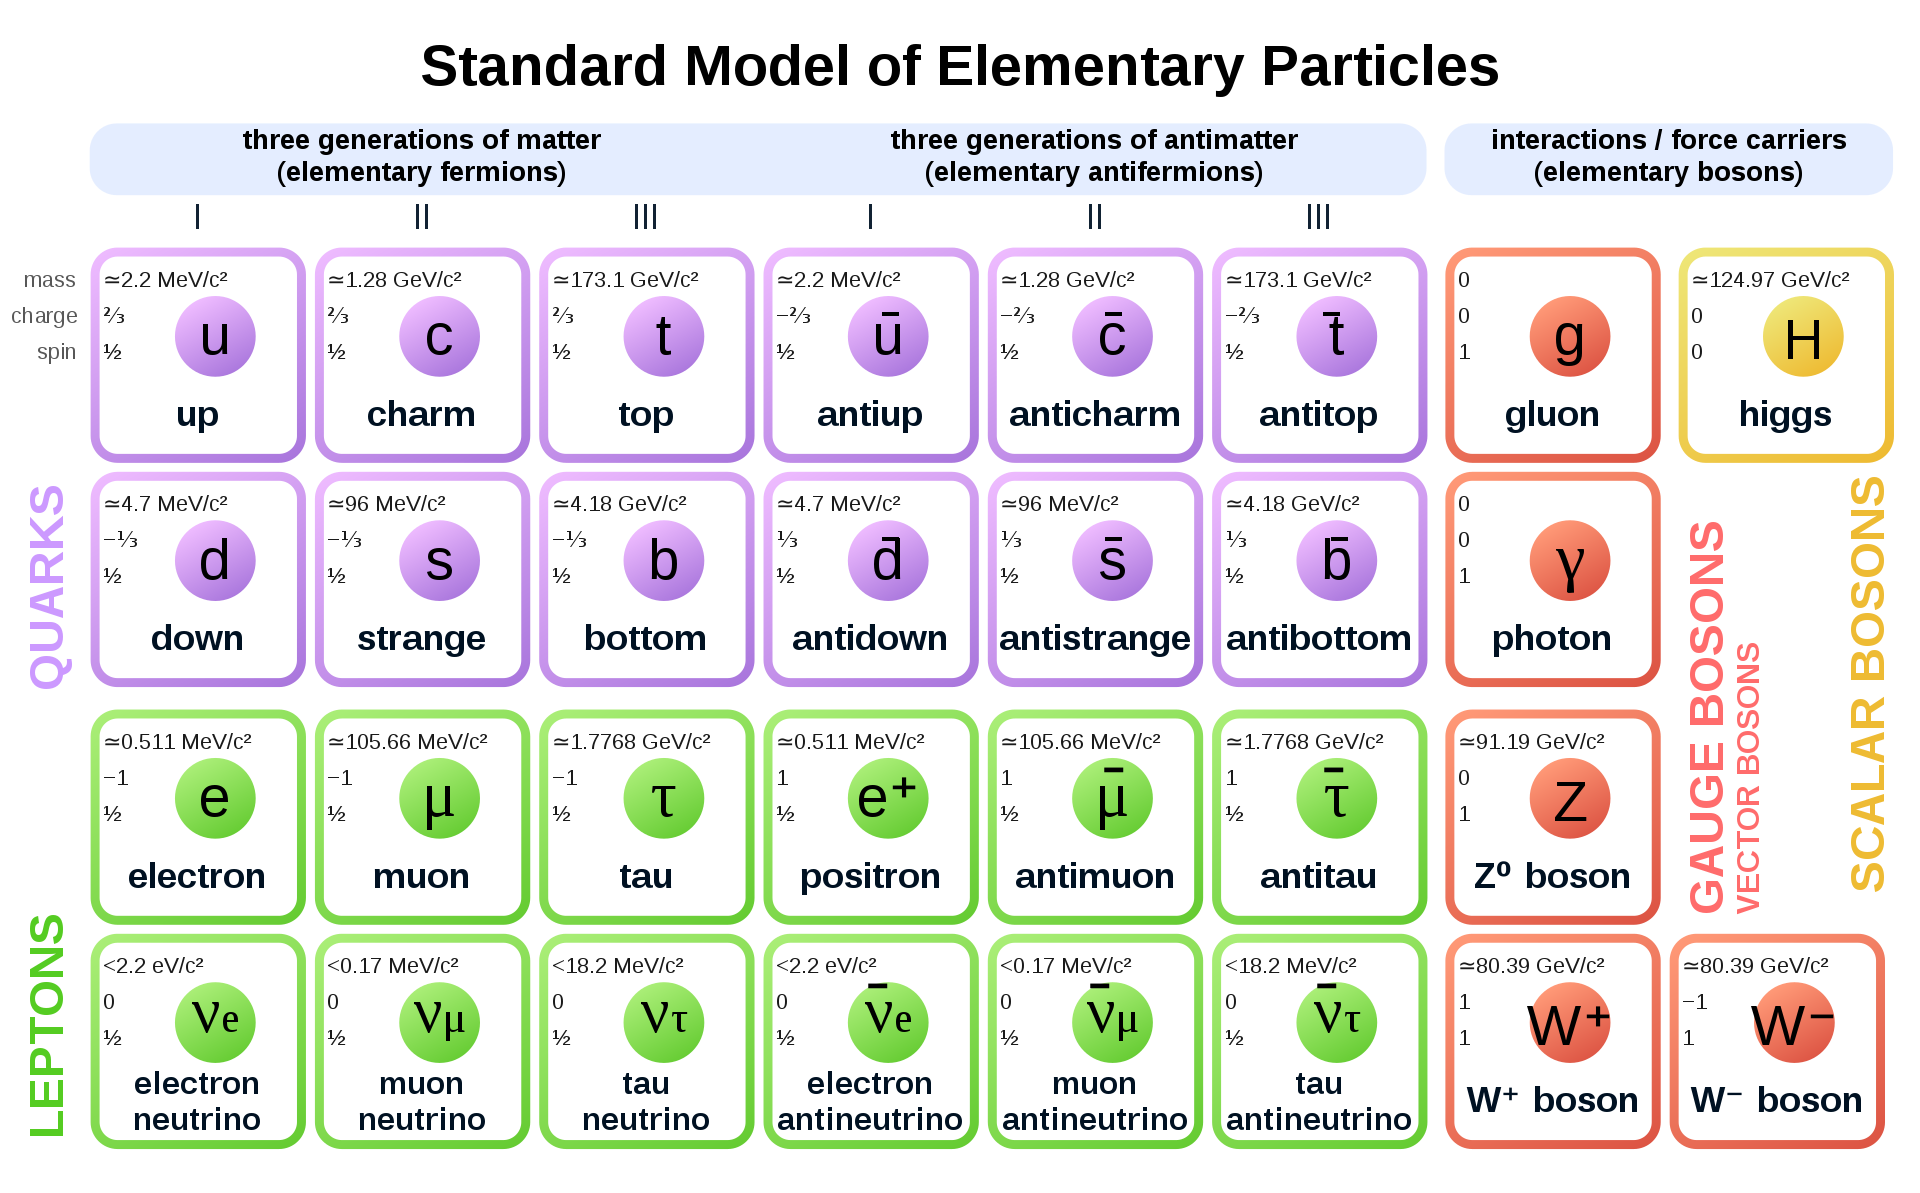
\includegraphics[width=1\textwidth]{figs/ch2/standard_model}
\caption{The Standard Model of Particle Physics. This displays all three generations of fermions 
in purple and green along with their antiparticle. On the right in red shows the force carrying
bosons along with the Higgs boson shown in yellow. Corresponding table of values can be 
found in Table \ref*{table:sm} on page \pageref*{table:sm}. }
\label{fig:sm_fig}
\end{figure}

\subsection{Theoretical Foundation}

The \gls{sm} represents a gauge theory that describes the strong, weak and electromagnetic interactions  
The \gls{sm} Lagrangian $\Lagr_{SM}$ can be broken down into two Lagrangians representing the strong interaction $\Lagr_{QCD}$
and the electroweak (\gls{ew})interaction $\Lagr_{EW}$. As in the name, the \gls{ew} theory is the combination of the electromagnetic 
and weak interactions. The Lagrangian $\Lagr_{SM}$ is invariant under local gauge transformations with the symmetry groups \cite{pich}.

\begin{equation}\label{eq:2.1} 
    \underbrace{SU(3)_{C}}_\text{QCD} \otimes \underbrace{SU(2)_{L} \otimes U(1)_{Y}}_\text{electroweak}
\tag{2.1}
\end{equation}
\\
The interactions between the strong, weak and electromagnetic forces are through the exchange of spin-1 gauge fields. For the strong field;
8 massless gluons. For the weak; 3 massive bosons, $W^\pm$ and $Z^0$. For the electromagnetic;
1 massless photon. The fermionic particles in Table \ref{table:sm} and Figure \ref{fig:sm_fig} can be represented
in a 3-fold family structure:
\\
\begin{equation}\label{eq:2.2}
  \begin{bmatrix}
    \nu_{e} & \textit{u} \\ 
    e^- & \textit{d}'
  \end{bmatrix}    
  ,
  \qquad
  \begin{bmatrix}
    \nu_{\mu} & \textit{c} \\
    \mu^- & \textit{s}'
  \end{bmatrix}
  ,
  \qquad
  \begin{bmatrix}
    \nu_{\tau} & \textit{t} \\
    \tau^- & \textit{b}'
  \end{bmatrix}
\tag{2.2}
\end{equation}
\\
where each quark appears in three different colors:
\\
\begin{equation}\label{eq:2.3}
    \begin{bmatrix}
        \nu_{\textit{l}} & \textit{q}_{u} \\
        \textit{l}^- & \textit{q}_{d}
    \end{bmatrix}
    \quad
    \equiv
    \quad 
    \begin{pmatrix}
        \nu_{\textit{l}} \\
        \textit{l}^-
    \end{pmatrix}_{L}
    ,
    \quad
    \begin{pmatrix}
        q_{\textit{u}} \\ 
        q_{\textit{d}} 
    \end{pmatrix}_{L}
    ,
    \quad
   l_{R}^-,\ q_{\textit{u}R},\ q_{\textit{d}R}
\tag{2.3}
\end{equation}
\\
plus their corresponding antiparticles. Here we see that the left-handed fields are 
$SU(2)_{L}$ doublets, whereas the right-handed partners transform as $SU(2)_{L}$ singlets.
 \par
 The vacuum-induced breakdown of gauge symmetry initiates Spontaneous Symmetry Breaking (\gls{ssb}) 
(as discussed later in section 2.2.3) within the \gls{ew} group, resulting in the emergence of the electromagnetic subgroup.
\\
 \begin{equation}\label{eq:2.4} 
    SU(3)_{C} \otimes SU(2)_{L} \otimes U(1)_{Y} \qquad \overrightarrow{\gls{ssb}} \qquad SU(3)_{C} \otimes U(1)_{QED} 
\tag{2.4}
\end{equation}
\\
The \gls{ssb} mechanism is the cause of the masses of the weak gauge bosons ($W^\pm$,$Z^0$) and gives rise 
to the appearance of a physical scalar boson in the \gls{sm} which can be seen as the yellow "Higgs" in 
Figure \ref{fig:sm_fig}. This also gives rise to the fermion masses and their mixings. These mixings keep track
of weak decays, i.e. one quark transitioning to another quark. These mixings were first formulated into 
a 6-quark model by Kobayashi and Maskawa by generalizing the Cabibbo matrix, creating the Cabibbo-Kobayashi-Maskawa (\gls{ckm}) matrix.
This matrix keeps track of weak decay rates in three generations of quarks \cite{ckm}.
\\
\begin{equation}\label{eq:2.5}
    \begin{bmatrix}
        d' \\
        s' \\
        b'
    \end{bmatrix}
    \quad
    =
    \quad
    \begin{bmatrix}
        V_{ud} & V_{us} & V_{ub} \\
        V_{cd} & V_{cs} & V_{cb} \\
        V_{td} & V_{ts} & V_{tb} \\
    \end{bmatrix}
    \begin{bmatrix}
        d \\
        s \\
        b \\
    \end{bmatrix}
\end{equation}
\\
Here we see on the left side are the weak interaction doublet partners of down-type quarks. On
the right side is the \gls{ckm} matrix along with a vector of mass eigenstates of down-type quarks.
The \gls{ckm} matrix states the probability of transitions between one quark flavor \textit{j} to another quark flavor \textit{i}.
These transitions are proportional to $|V_{ij}|^2$. 
\\
\begin{equation}\label{eq:2.6}
    \medmath{
    \begin{bmatrix}
        |V_{ud}| & |V_{us}| & |V_{ub}| \\
        |V_{cd}| & |V_{cs}| & |V_{cb}| \\
        |V_{td}| & |V_{ts}| & |V_{tb}| 
    \end{bmatrix}
    =
    \begin{bmatrix}
       0.97373 \pm 0.00031 & 0.2243 \pm 0.0008 & 0.00382 \pm 0.00020 \\
       0.221 \pm 0.004 & 0.975 \pm 0.006 & 0.0408 \pm 0.0014 \\
       0.0086 \pm 0.0002 & 0.0415 \pm 0.0009 & 1.014 \pm 0.029 \\ 
    \end{bmatrix}
    }
\tag{2.6}
\end{equation}
\\
Here we see in Eq. \ref{eq:2.6} the most recent transition probabilities as stated 
by the Particle Data Group (\gls{pdg}) \cite{workman}. Now, we expect unitary of the \gls{ckm} 
matrix but if we check it, even in the first row, we see:
\\
\begin{equation}\label{eq:2.7}
    |V_{ud}|^2 \ + |V_{us}|^2 \ + |V_{ub}|^2 \ = \ 0.9985 \pm 0.0007
\tag{2.7}
\end{equation}
\\
The difference from the theoretical unitary value of 1 has a standard deviation of 2.2$\sigma$ which 
this gives an exciting strong indication of physics Beyond the Standard Model or \gls{bsm}. 
\\
\subsection{Fundamental Interactions}
\subsubsection{The Electromagnetic Interaction}

Quantum Electrodynamics (\gls{qed}) is the foundational knowledge of electromagnetism. All charged particles
communicate with each other through the electromagnetic force carrier boson called the Photon. \gls{qed} is a 
consequence of the $U(1)$ symmetry. It is the separated force from the \gls{ew} interactions and can be seen 
in Eq. \ref{eq:2.1} as $U(1)_{em}$. In order to obtain the \gls{qed} Lagrangian, let's look at the dynamics of
a free $1/2$ spin fermion.
%
\begin{equation}\label{eq:2.8}
    \Lagr_{0} = \bar{\psi}(i\gamma^{\mu}-m)\psi
\tag{2.8}
\end{equation}
%
In Eq. \ref{eq:2.8} notation-wise, $\psi$ is the Dirac Spinor, $m$ is the mass and the Dirac matrices are 
denoted by $\gamma^{\mu} \cdot \bar{\psi} = \psi^{\dag} \; \gamma^{0}$ which is also known as the Dirac adjoint.
In the Lagrangian, the $\gamma^{\mu}$ are the Dirac $4 \ \times \ 4$ matrices and can be seen in Eq. \ref{eq:2.9}.
%
\begin{equation}\label{eq:2.9}
    \gamma^{0}=
    \begin{bmatrix}
        0 \ \ & I \\
        -I \ \ & 0 \\
    \end{bmatrix}
    ,
    \quad
    \gamma^{i}=
    \begin{bmatrix}
        0  & \sigma^{i} \\
        -\sigma^{i} & 0 \\
    \end{bmatrix}
    ,
    \quad
    \gamma^{5}=
    \begin{bmatrix}
        -I \ \ & 0 \\
        0 \ \ & I \\
    \end{bmatrix}
\tag{2.9}    
\end{equation}
%
These are written in terms of the Pauli matrices which are shown in Eq. \ref{eq:2.10}.
%
\begin{equation}\label{eq:2.10}
    \sigma^{1}=
    \begin{bmatrix}
       \ 0 \ \ \  \ & 1 \ \\
       \ 1 \ \ \  \ & 0 \ \\
    \end{bmatrix}
    ,
    \quad
    \sigma^{2}=
    \begin{bmatrix}
        0  \ \  & i \ \\
        -i \ \  & 0 \ \\
    \end{bmatrix}
    ,
    \quad
    \sigma^{3}=
    \begin{bmatrix}
       \ 1 \  \ & 0 \ \\
       \ 0 \  \ & -1 \ \\
    \end{bmatrix}
\tag{2.10}
\end{equation}
%
The Lagrangian in Eq. \ref{eq:2.8} is invariant under global gauge transformations, but is 
not invariant under local $U(1)$ transformations. In order to induce local invariance under transformations,
as shown in Eq. \ref{eq:2.11}, an additional vectorial gauge field that is massless is required.
%
\begin{equation}\label{eq:2.11}
    \psi(x) \rightarrow \psi'(x) = e^{i\alpha(x)}\psi(x)  
\tag{2.11}
\end{equation}
%
The gauge field that is required is denoted as $A_{\mu}(x)$ and is shown in eq \ref{eq:2.12}.
Additionally, the covariant derivative $D_{\mu}(x)$ is shown in Eq. \ref{eq:2.13}.
%
\begin{equation}\label{eq:2.12}
    A_{\mu}(x) \rightarrow A_{\mu}'(x) = A_{\mu}(x) \ + \ \frac{1}e\partial_{\mu}\alpha(x)
\tag{2.12}    
\end{equation}
%
\begin{equation}\label{eq:2.13}
    D_{mu}(x) = \partial_{mu} \ - \ ieA_{\mu}(x)
\tag{2.13}
\end{equation}
%
Using these two fields, the field strength tensor can be expressed in Eq. \ref{eq:2.14}.
%
\begin{equation}\label{eq:2.14}
    F_{\mu\nu} = \partial_{\mu}A_{\nu} \ - \ \partial_{\nu}A_{\mu}
\tag{2.14} 
\end{equation}
%
Now that local $U(1)$ symmetry is applied, Eq. \ref{eq:2.11} can be used along with Eq. \ref{eq:2.14}
to express the \gls{qed} Lagrangian. This is shown in Eq. \ref{eq:2.15}.
%
\begin{equation}\label{eq:2.15}
    \Lagr = \bar{\psi}i\gamma^{\mu}-m)\psi \ - \ \frac{1}4F_{\mu\nu}F^{\mu\nu}
\tag{2.15}
\end{equation}
%
From here, the interaction term called the electromagnetic charge current density $j^{\mu}$
is added to Eq. \ref{eq:2.15}. This equation is defined in Eq. \ref{eq:2.16}. 
%
\begin{equation}\label{eq:2.16}
    j^{\mu} = \bar{\psi}\gamma^{\mu}\psi
\tag{2.16}
\end{equation}
%
putting both of these equations together we get Eq. \ref{eq:2.17}.
%
\begin{equation}\label{eq:2.17}
    \Lagr = \underbrace{\bar{\psi}i\gamma^{\mu}-m)\psi}_\text{free Lagrangian} \ \ \ -  \underbrace{ej^{\mu}A_{\mu}}_\text{interaction term}  - \ \ \ \underbrace{\frac{1}4F_{\mu\nu}F^{\mu\nu}}_\text{kinetic term}
\tag{2.17}
\end{equation}
%
Here, Eq. \ref{eq:2.17} is the \gls{qed} Lagrangian. According to Noether's theorem which states 
that every differentiable symmetry of the action of a physical system with conservative forces has
a corresponding conservation law \cite{noether}. For QED, this conserved quantity is the electromagnetic 
charge \textit{q}. The \gls{qed} Lagrangian thus shows the relationship between the photon field $A_{\mu}$ 
and the Dirac fields $\psi$ which emerged as a consequence of $U(1)$ symmetry.
%

\subsubsection{The Electroweak Interaction}

The \gls{ew} force is the combination of the electromagnetic interaction and the weak interaction.
Both of these forces appear differently in low energies but they happen to combine at much higher
energies. Thus, this theory models them as two different aspects of the same force. The predicted 
unification energy is on the order of 246 Gev or on a temperature scale of approximately $10^{15} K$. 
This implies that the two forces coexisted at the start of the Big Bang and later diverged during 
the Quark Epoch, occurring approximately $10^{-12}$ seconds after the inception of the Big Bang.
\par
The mathematical formulation is found within the $SU(2)_{L}$ symmetry group in Eq. \ref{eq:2.1}. 
Weak isospin and weak hypercharge are quantum numbers relating the electrically charged part of the weak interaction and are 
labeled $T_{\textit{i}}$ and $Y_{W}$ respectively. These are known as generators of $SU(2)$ and $U(1)$ and give rise to the gauge
bosons that mediate this force. Once \gls{ssb} occurs, these bosons are seen in the \gls{sm} as the $W^{\pm}$, 
$Z^{0}$, and the photon. The conserved quantity within the electroweak force is the third component of the generator 
$T_{\textit{i}}$, quantum number $T_{3}$. However, interaction with the Higgs field do not conserve weak isospin $T_{3}$
and thus causing fermion mixings as seen in the \gls{ckm} matrix in \ref{eq:2.6}. Though, there are specific combinations
of them that do not interact with the Higgs field and therefore are conserved, this happens to be the electric charge \textit{q}.
The combinations that give rise to \textit{q} are given by Eq. \ref{eq:2.18}.
%
\begin{equation}\label{eq:2.18}
    Q = T_{3} + \frac{1}2Y_{W}
\tag{2.18}
\end{equation}
%
The \gls{ew} force is \textit{chiral}, which requires treating both components of the fermionic fields $\psi$ separately.
Left-handed fermions have weak isospin of $T_{3}=\pm 1/2$ and are represented by doublets $\psi_{L}$. Whereas right-handed
fermions have weak isospin of $T_{3} = 0$ and are represented by singlets $\psi_{R}$. Both components behave differently under
$SU(2)_{L}$ and $U(1)_{\gamma}$ local transformations. A quick formulation of the \gls{ew} Lagrangian can be formulated
by introducing the covariant derivative acting on both the left-handed fermionic field (Eq. \ref{eq:2.19}) and the right-handed
fermionic field (Eq. \ref{eq:2.20}).
%
\begin{equation}\label{eq:2.19}
    D_{\mu}\psi_{L}=(\partial_{\mu} \ + \ ig\frac{\sigma_{i}}2W_{\mu}^{i} \ + \ ig'\frac{\gamma}2B_{\mu}^{i})\psi_{L}
\tag{2.19}
\end{equation}
%
\begin{equation}\label{eq:2.20}
    D_{\mu}\psi_{R}=(\partial_{\mu} \ + \  ig'\frac{\gamma}2B_{\mu}^{i})\psi_{R}
\tag{2.20}
\end{equation}
%
Here we see the Pauli matrices $\sigma$ that are shown in Eq. \ref{eq:2.10}, $g$ and $g'$ are coupling constants for 
the $W^{i}$ and $B_{\mu}$ boson field strength tensors which are shown in Eq. \ref{eq:2.21} and Eq. \ref{eq:2.22}.
%
\begin{equation}\label{eq:2.21}
    B_{\mu\nu} = \partial_{\mu}B_{\nu} \ - \ \partial_{\nu}B_{\mu}
\tag{2.21}
\end{equation}
%
\begin{equation}\label{eq:2.22}
    W^{i}_{\mu\nu} = \partial_{\mu}W^{\nu}_{i} \ - \ \partial_{\nu}W^{\mu}_{i} \ - \ \epsilon_{ijk} W^{\mu}_{j}G^{\nu}_{k}
\tag{2.22}
\end{equation}
%
With these, the electroweak Lagrangian can be assembled as shown in Eq. \ref{eq:2.23} where the sum over $j$ covers the $L$
doublet and two $R$ singlets.
%
\begin{equation}\label{eq:2.23}
    \Lagr_{EW} =  \sum_{j=1}^{3}\bar{\psi_{j}}[i\gamma^{\mu}D_{\mu}]\psi_{j} \ - \ \frac{1}4W_{i}^{\mu\nu}W_{\mu\nu}^{i} \ - \ \frac{1}4B^{\mu\nu}B_{\mu\nu}  
\tag{2.23}
\end{equation}
%
Both, $W^{\pm}$ bosons arise from linear combinations between $W_{1}$ and $W_{2}$ as shown in Eq. \ref{eq:2.24}.
%
\begin{equation}\label{eq:2.24}
    W^{\pm} = \frac{1}{\sqrt{2}}(W_{1} \mp iW_{2})
\tag{2.24}
\end{equation}
%
Finally, the application of a rotation by an angle $\theta_{W}$ allows the restoration of the massless vector field $A$ that's 
associated with the photon and the massive weak neutral $Z^{0}$. Here, $\theta_{W}$ represents the \textit{weak mixing angle}. This 
rotation introduces the mismatch between the $W^{\pm}$ bosons and the $Z^{0}$ boson. Through \gls{ssb}, the two bosons (photon and $Z^{0}$)
become physical with different masses given by Eq. \ref{eq:2.25}.
%
\begin{equation}\label{eq:2.25}
    \begin{pmatrix}
        \gamma \\
        Z^{0} \\
    \end{pmatrix}
    =
    \begin{pmatrix}
        cos\theta_{W} & sin\theta_{W} \\ 
        -sin\theta_{W} & cos\theta_{W} \\
    \end{pmatrix}
    \begin{pmatrix}
        B \\
        W_{3} \\
    \end{pmatrix}
\tag{2.25}
\end{equation}
%
where the offset of the $Z^{0}$ mass from the $W^{\pm}$ bosons can be given by Eq. \ref{eq:2.26}.
%
\begin{equation}\label{eq:2.26}
    m_{Z} = \frac{m_{W}}{cos\theta_{W}}
\tag{2.26}
\end{equation}
%
A pictorial representation of this \textit{weak mixing angle} showing the pattern of weak 
isospin, $T_{3}$, and weak hypercharge, $Y_{W}$, of the known elementary particles can be seen 
in Figure \ref{fig:wma}. 
%
\newpage
\begin{figure}[ht]
    \centering
    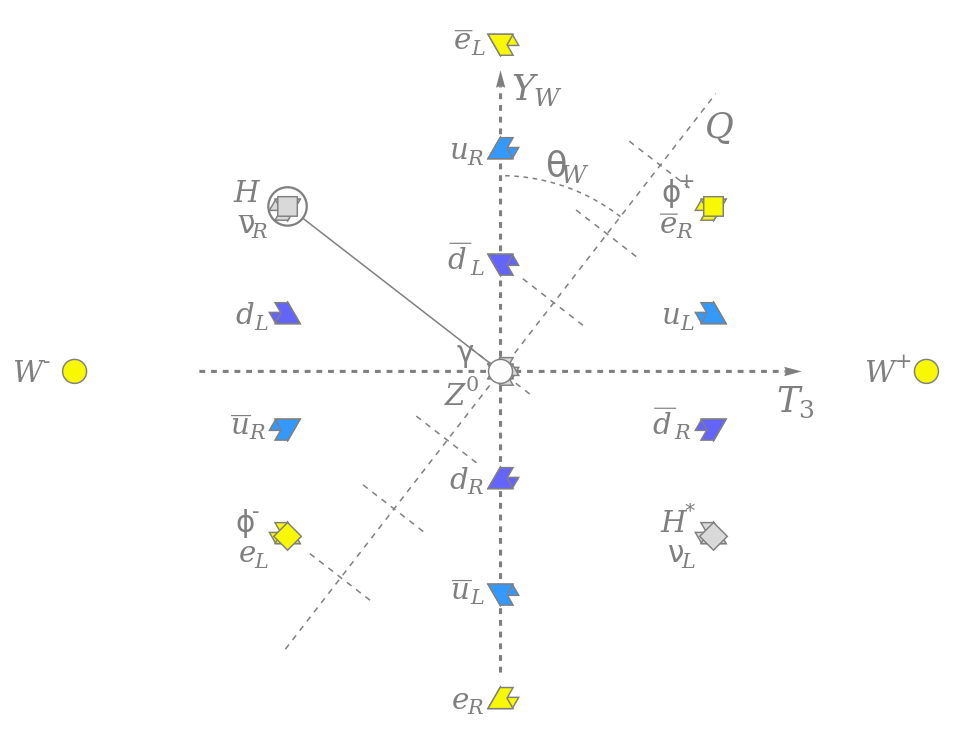
\includegraphics[scale=0.55]{figs/ch2/weak_mixing_angle}%width=14cm, height=14cm
    \caption{ The pattern of weak isospin, $T_{3}$, and weak hypercharge, $Y_{W}$, of the known elementary particles.
    The electric charge is shown as $Q$ along the \textit{weak mixing angle}. The neutral Higgs field is seen being
    circled, this field breaks the electroweak symmetry and interacts with other particles, giving them mass. }
\label{fig:wma}
\end{figure}


\subsubsection{The Strong Interaction}

The strong interaction, or the strong force, is the fundamental force that confines quarks, forming hadrons.
It is also the reason why nuclei are able to bind inside the nucleus forming atomic nuclei. 
To model the strong interaction, Quantum Chromodynamics, i.e. \gls{qcd}, is used. This theory was founded on 
Yang-Mills theory \cite{yang-mills}, which extends \gls{qed}, adding the non-abelian symmetry group $SU(3)$. 
Quarks interact with gluons and each other by way of a type of charge called the color charge. Unlike the 
electromagnetic charge, color charges comes with three types ($\pm$red, $\pm$green, $\pm$blue) which dictates
the rules of behavior. Due to the strength of this force, when hadrons collide with high energy particles, jets of massive particles are produced instead of emitting their constituents as separate particles. 
\par
In the symmetry group $SU(3)$ Lie algebra, there are eight generators, therefore just as many gauge fields need to 
be introduced. The associated fermionic fields are represented by three-dimensional vectors, i.e. triplets, where 
each component represents color charges. Matrices called the Gell-Mann matrices $t_{a}$ are used to represent 
the generators, having the commutation relationship: $[t_{a},t_{b}]=if_{abc}t_{c}$.
Under a transformation $U(x)$, the quark field $\psi$ behaves as stated in Eq. \ref{eq:2.27}.
%
\begin{equation}\label{eq:2.27}
    \psi(x) \rightarrow \psi'(x) = U(x)\psi = e^{i\alpha_{a}(x)t_{a}}\psi
\tag{2.27}    
\end{equation}
% 
Similarly to the \gls{qed}'s case, new fields are introduced: the gluon field $G^{a}_{\mu}$ and 
a covariant derivative, as seen in Eq. \ref{eq:2.28}.
%
\begin{equation}\label{eq:2.28}
    D_{\mu} = \partial_{\mu} + ig_{s}t_{a}G^{a}_{\mu}
\tag{2.28}
\end{equation}
%
The gluon field behavior has requirements under the transformation $U(x)$. These 
requirements are shown in Eq. \ref{eq:2.29}.
%
\begin{equation}\label{eq:2.29}
    G^{a}_{\mu} \rightarrow G'^{a}_{\mu} = U(x)G^{a}_{\mu}t^{a}U^{\dagger}(x) + \frac{i}g_{s}(d_{\mu}U(x))U^{\dagger}(x)
\tag{2.29}
\end{equation}
%
The field strength tensor for the gluon field $G^a_{\mu}$ that follows the requirements as stated 
in Eq. \ref{eq:2.29} is shown in Eq. \ref{eq:2.30}.
%
\begin{equation}\label{eq:2.30}
    G^{\mu\nu}_{a} = \partial_{\mu}G^{\nu}_{a} - \partial_{\nu}G^{\mu}_{a} - g_{s}f_{abc}G^{\mu}_{b}G^{\nu}_{c}
\tag{2.30}
\end{equation}
%
Lastly, the \gls{qcd} Lagrangian density, using the previously shown equations, can be derived 
and is shown in Eq. \ref{eq:2.31}.
%
\begin{equation}\label{eq:2.31}
    \Lagr_{QCD} = \bar{\psi}(i\gamma^{\mu}D_{\mu} - m)\psi - \frac{1}4G^{\mu\nu}_{a}G^{a}_{\mu\nu}
\tag{2.31}
\end{equation}
%
Here, we see a noteworthy aspect of the \gls{qcd} Lagrangian which is the self interaction between 
gluons due to having color charge. 

\subsection{Spontaneous Symmetry Breaking}

The gauge symmetries of the \gls{sm} ($SU(3)_{C}$, $SU(2)_{L}$, $SU(1)_{\gamma}$) have proven to 
be successful in predicting interactions between its particles. But particles have masses (besides the photon)!
So far, there has been no references to any mass terms within these symmetries. Another mechanism 
was needed in order to allow generation of masses within these gauge theories. This mechanism is called 
spontaneous symmetry breaking (\gls{ssb}).
\par
Suppose there is a scalar field $\phi$ with a corresponding Lagrangian.
%
\begin{equation}\label{eq:2.32}
    \Lagr = \frac{1}2(\partial_{\mu}\phi)(\partial^{\mu}\phi)+e^{-(\alpha\phi)^{2}}
\tag{2.32}
\end{equation}
%
There is no obvious mass term within this Lagrangian, but if the exponential is expanded, we get:
%
\begin{equation}\label{eq:2.33}
    \Lagr = \frac{1}2(\partial_{\mu}\phi)(\partial^{\mu}\phi)+1-\alpha^{2}\phi^{2}+\frac{1}2\alpha^{4}\phi^{4}-\frac{1}6\alpha^{6}\phi^{6}+ \ ...
\tag{2.33}
\end{equation}
%
Here, the 1 is irrelevant, but the second term is close to the known mass term within the Klein-Gordon equation, with $\alpha^{2} = \frac{1}2(mc/\hbar)^{2}$, while the higher 
order terms correspond to coupling terms. The Lagrangian describes a particle of mass: 
%
\begin{equation}\label{eq:2.34}
    m=\sqrt{2}\alpha\hbar/c
\tag{2.34}
\end{equation}
%
Now that the hidden mass term can be found within a Lagrangian for a field, suppose there's a Lagrangian 
that takes the form: 
%
\begin{equation}\label{eq:2.35}
    \Lagr = \frac{1}2(\partial_{\mu}\phi)(\partial^{\mu}\phi)+\frac{1}2\mu^{2}\phi^{2}-\frac{1}4\lambda^{2}\phi^{4}
\tag{2.35}
\end{equation}
%
Here the second term looks like the mass term as previously discussed be we see that the sign is flipped and 
therefore would be imaginary. In order to properly understand this, Feynman calculus must be used which 
treats this more like a perturbation procedure which is started from the ground state, or vacuum. We must represent this 
Lagrangian classically, as seen in \ref{eq:2.36}, in order to obtain the minimum.
%
\begin{equation}\label{eq:2.36}
    \Lagr = \textit{T} - \textit{U}
\tag{2.36}
\end{equation}
%
We obtain the minimum:
%
\begin{equation}\label{eq:2.37}
    \textit{U}(\phi) = -\frac{1}2\mu^{2}\phi^{2}+\frac{1}4\lambda^{2}\phi^{4}
\tag{2.37}
\end{equation}
%
We see that the minimum occurs at:
%
\begin{equation}\label{eq:2.38}
    \phi = \pm\mu/\lambda
\tag{2.38}
\end{equation}
%
A new variable, $\eta$, must be introduced which represents a perturbation around this ground state.
%
\begin{equation}\label{eq:2.39}
    \eta \equiv \phi \pm \frac{\mu}\lambda
\tag{2.39}
\end{equation}
%
Now, to rewrite the Lagrangian in Eq. \ref{eq:2.35} in terms of $\eta$.
%
\begin{equation}\label{eq:2.40}
    \Lagr = \frac{1}2(\partial_{\mu}\eta)(\partial^{\mu}\eta)-\mu^{2}\eta^{2}\pm\mu\lambda\eta^{3}-\frac{1}4\lambda^{2}\eta^{4} + \frac{1}4(\mu^{2}/\lambda)^{2}
\tag{2.40}
\end{equation}
%
The second term is now the correct sign for the mass term! The mass of the particle from the Lagrangian is:
%
\begin{equation}\label{eq:2.41}
    m = \sqrt{2}\mu\hbar/c
\tag{2.41}
\end{equation}
%
Where the third and fourth term are corresponding coupling terms. Figure \ref{fig:2d_potential} shows 
the shape of the potential $U(\phi)$ and its minima. 
%
\begin{figure}[h]
    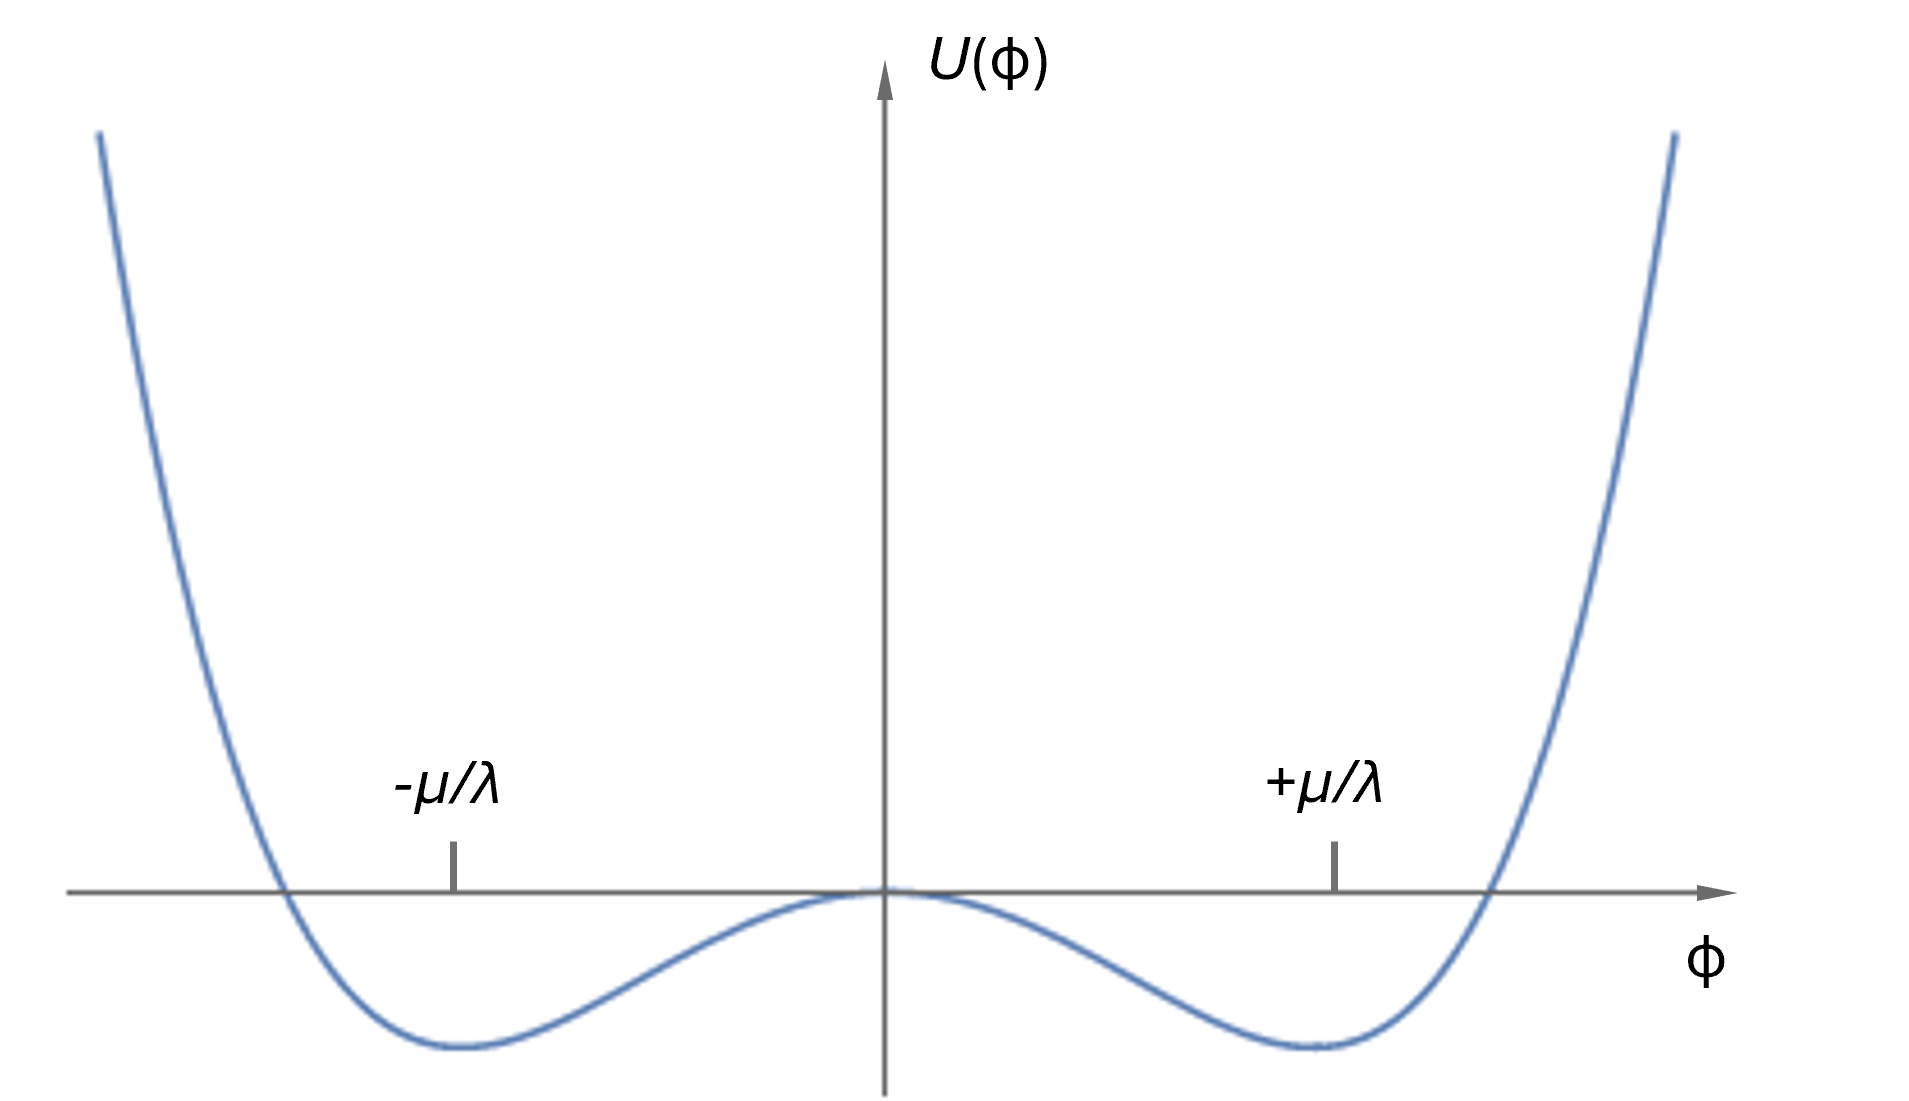
\includegraphics[width=0.8\linewidth,height=8cm]{figs/ch2/2d_potential.png}
    \centering
\caption{Graph of $\textit{U}(\phi)$ in Eq. \ref{eq:2.37}}
\label{fig:2d_potential}
\end{figure}
 %   
This example illustrates \gls{ssb}, though it may not be too obvious. The Lagrangian in Eq. \ref{eq:2.40}
is the same as Eq. \ref{eq:2.35} except for one thing, its symmetry is broken. The Lagrangian in 
Eq. \ref{eq:2.35} is \textit{even} in $\phi$, as in, it's invariant ($\phi \rightarrow -\phi$).
Whereas the Lagrangian in \ref{eq:2.40} is not, thus \gls{ssb}. This happens due to the fact that the chosen state,
i.e. the ground state, does not share this symmetry. However, the collection of all states does share this 
symmetry. This example shows a broken \textit{discrete} symmetry, i.e left or the right side in Figure \ref{fig:2d_potential}.
To make this more physical, let's consider a Lagrangian containing continuous symmetries that demonstrates \gls{ssb}. 
%
\begin{equation}\label{eq:2.42}
    \Lagr = \frac{1}2(\partial_{\mu}\phi_{1})(\partial^{\mu}\phi_{1}) + \frac{1}2(\partial_{\mu}\phi_{2})(\partial^{\mu}\phi_{2}) + \frac{1}2\mu^{2}(\phi^{2}_{1}+\phi^{2}_{2})-\frac{1}4\lambda^{2}(\phi^{2}_{1}+\phi^{2}_{2})^{2}
\tag{2.42}
\end{equation}
%
Now this has two fields, $\phi_{1}$ and $\phi_{2}$, and only contains sum of squares, therefore it is invariant under
\textit{rotations} in $\phi_{1}$, $\phi_{2}$ space. The potential $U(\phi_{1},\phi_{2})$ is then:
%
\begin{equation}\label{eq:2.43}
    \textit{U}(\phi_{1},\phi_{2}) = -\frac{1}2\mu^{2}(\phi^2_{1}+\phi^2_{2})+\frac{1}4\lambda^{2}(\phi^{2}_{1}+\phi^{2}_{2})^{2}
\tag{2.43}
\end{equation}
%
and the minima lie on the circle of radius $\mu/\lambda$:
%
\begin{equation}\label{eq:2.44}
    \phi^{2}_{1}+\phi^{2}_{2} = \mu^{2}/\lambda^{2}
\tag{2.44}
\end{equation}
%
Now in order to apply Feynman calculus as we did previously, we must expand around a particular ground state or vacuum.
%
\begin{equation}\label{eq:2.45}
    \phi_{1} = \mu/\lambda: \\ \phi_{2} = 0
\tag{2.45}
\end{equation}
%
\begin{figure}[h]
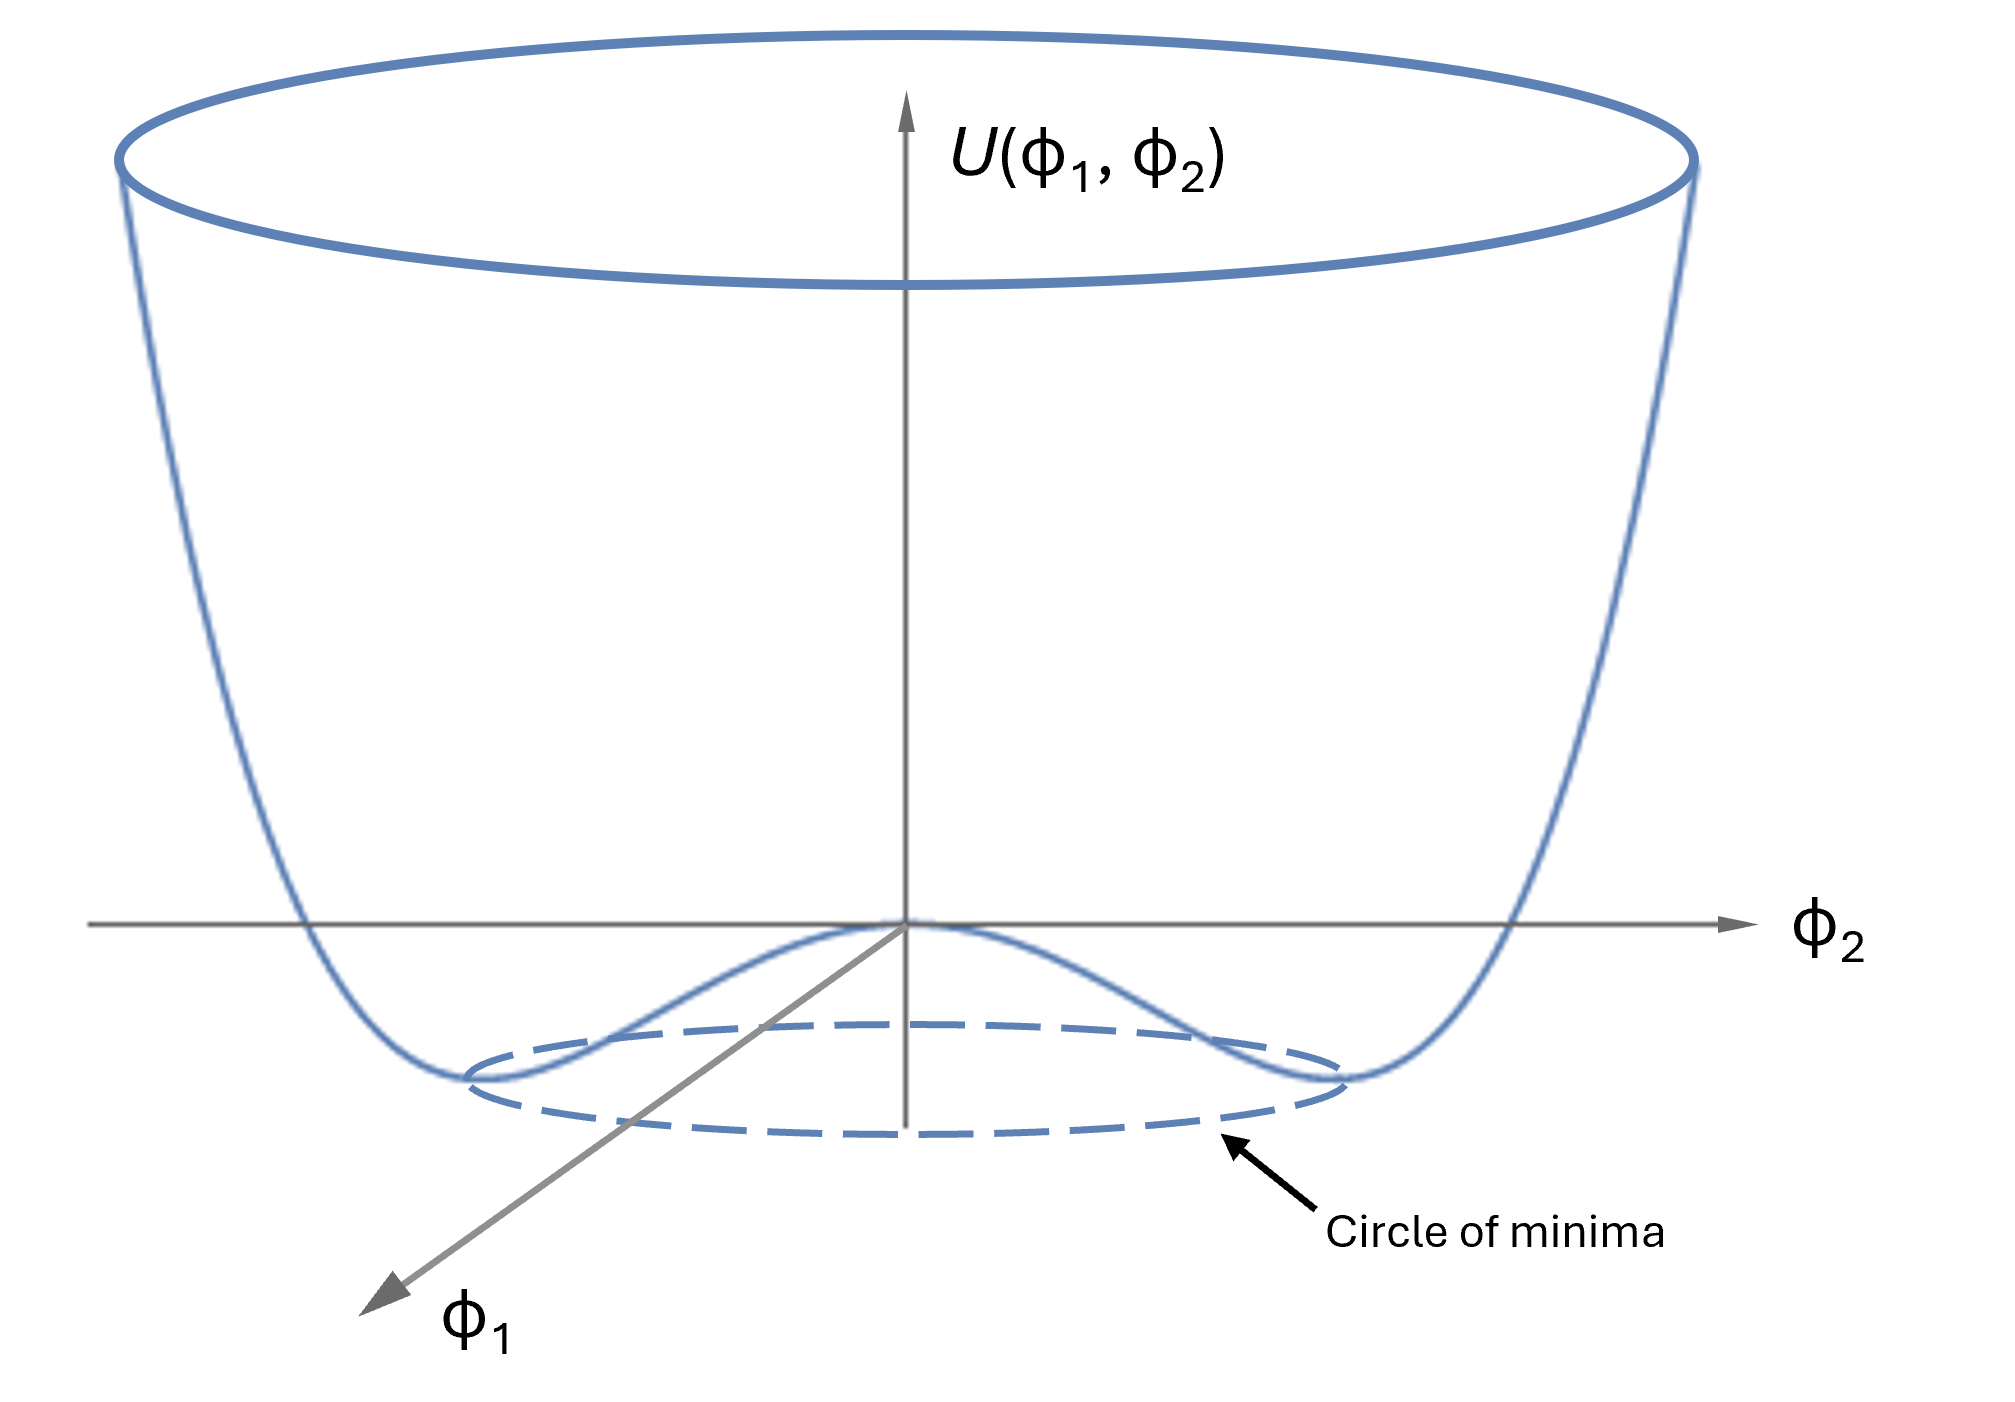
\includegraphics[width=0.8\linewidth,height=8cm]{figs/ch2/3d_pot_graph2.png}
\centering
\caption{Graph of $\textit{U}(\phi_{1},\phi_{2})$ in Eq. \ref{eq:2.43}}
\label{fig:3d_pot_graph2}
\end{figure}
%
Following the steps shown above, we introduce new fields that represent fluctuations around the vacuum.
%
\begin{equation}\label{eq:2.46}
    \eta \equiv \phi_{1}-\mu/\lambda; \qquad \nu \equiv \phi_{2}
\tag{2.46}
\end{equation}
%
Rewriting the Lagrangian from Eq. \ref{eq:2.42} using these new fields:
%
\begin{equation}\label{eq:2.47}
\begin{split}
    \Lagr = &[\frac{1}2(\partial_{\mu}\eta\partial^{\mu}\eta)  - \mu^{2}\eta^{2}] + [\frac{1}2(\partial_{\mu}\nu\partial^{\mu}\nu)] \ - \ \\  
    &[\mu\lambda(\eta^{3} + \eta\nu^{2}) + \frac{\lambda^{2}}4(\eta^{4}+\nu^{4}+2\eta^{2}\nu^{2})] + \frac{\mu^{4}}{4\lambda^{2}}
\end{split}
\tag{2.47}
\end{equation}
%
The first term is the free Klein-Gordon Lagrangian for the field $\eta$, carrying a mass of:
%$\qquad \qquad \qquad \qquad \qquad \qquad \qquad \quad \ \ \ $
\begin{equation}\label{eq:2.48}
    m_{\eta} = \sqrt{2}\mu\hbar/c
\tag{2.48}
\end{equation}
%
The second term is a free Lagrangian for the field $\nu$, which is massless:
%
\begin{equation}\label{eq:2.49}
    m_{\nu} = 0
\tag{2.49}
\end{equation}
%
The third and fourth term show five different couplings. An important phenomena that occurs here is that 
one of the two fields is \textit{massless}. This is to be expect since \gls{ssb} of a continuous symmetry 
is always accompanied by one or more massless scalar (spin-0) particles, these are called Goldstone Bosons.
At first glance this may seem like an issue since there are no massless scalar bosons within the \gls{sm}.
At this point, another mechanism is needed to extract masses. This mechanism is called the Higgs Mechanism \cite{Higgs}.

\subsection{The Higgs Mechanism}

This mechanism has been one of the most influential additions to the \gls{sm} and is embodied by the Higgs boson. The 
combination of \gls{ssb} and local gauge invariance has given way to the mechanism that has since accurately predicted
masses for gauge fields, explaining the massive bosons $W^{\pm}$ and $Z^{0}$.

To start, the Lagrangian in Eq. \ref{eq:2.35} must be written with the combination of two fields,
$\phi_{1}$ and $\phi_{2}$ into a complex field:
%
\begin{equation}\label{eq:2.50}
    \phi \equiv \phi_{1} + \textit{i}\phi_{2}
\tag{2.50}
\end{equation}
%
It is written like this so that its minima lie on a circle as seen in Figure \ref{fig:3d_pot_graph2}:
%
\begin{equation}\label{eq:2.51}
    \phi^{*}\phi = \phi^{2}_{1} +\phi^{2}_{2}
\tag{2.51}
\end{equation}
%
The Lagrangian in Eq. \ref{eq:2.35} can be rewritten as:
%
\begin{equation}\label{eq:2.52}
    \Lagr = \frac{1}2(\partial_{\mu}\phi)^{*}(\partial^{\mu}\phi)+\frac{1}2\mu^{2}(\phi^{*}\phi)-\frac{1}4\lambda^{2}(\phi^{*}\phi)^{2}
\tag{2.52}
\end{equation}
%
Now the trick here is to not only introduce a massless gauge field $A^{\mu}$, but the partial derivatives are replaced with 
\textit{covariant} derivatives.
%
\begin{equation}
    \mathfrak{D} = \partial_{\mu} + i\frac{q}{\hbar c}A_{\mu}
\end{equation}
%
Rewriting Eq. \ref{eq:2.52}:
%
\begin{equation}\label{eq:2.53}
\begin{split}
    \Lagr = &\frac{1}2[(\partial_{\mu} - i\frac{q}{\hbar c}A_{\mu})\phi]^{*}[(\partial^{\mu} + i\frac{q}{\hbar c}A^{\mu})\phi] \ + \\ 
    &\frac{1}2\mu^{2}(\phi^{*}\phi)  -  \frac{1}4\lambda^{2}(\phi^{*}\phi)^{2}  - \frac{1}{16\pi}F^{\mu\nu}F_{\mu\nu}
\end{split}
\tag{2.53}
\end{equation}
%
Now to define two new fields in order to fluctuate about the ground state.
%
\begin{equation}\label{eq:2.54}
    \eta = \phi_{1} \ - \ \mu/\lambda; \qquad \xi = \phi_{2}
\tag{2.54}
\end{equation}
%
Once these fields are substituted and the Lagrangian is expanded, it will output a mass term but will also include a bilinear interaction and 
a massless Goldstone boson. To do away with the useless nonsense, a clever trick can be implemented.
The complex field can be rewritten in terms of its real and imaginary parts as shown:
%
\begin{equation}\label{eq:2.55}
\begin{split}
    \phi  \ \rightarrow  \ \phi' \  &= \ (cos\theta + \textit{i}sin\theta)(\phi_{1}+\textit{i}\phi_{2}) \\
    \phi' \ &= \ (\phi_{1}cos\theta - \phi_{2}sin\theta) \ + \ \textit{i}(\phi_{1}sin\theta+\phi_{2}cos\theta) 
\end{split}
\tag{2.55}
\end{equation}
%
If $\theta$ is picked as: 
%
\begin{equation}\label{eq:2.56}
    \theta = -\tan^{-1}(\phi_{2}/\phi_{1})
\tag{2.56}
\end{equation}
%
It will ensure that $\phi'$ is real and that the second field, $\xi$, is dropped. Now the 
Lagrangian in Eq. \ref{eq:2.53} can be expanded out to get the final result.
%
\begin{equation}\label{eq:2.57}
\begin{split}
    \Lagr  = &[\frac{1}2(\partial_{\mu}\eta)(\partial^{\mu}\eta)-\mu^{2}\eta^{2}] \ + \ [-\frac{1}{16\pi}F^{\mu\nu}F_{\mu\nu}+\frac{1}2(\frac{q}{\hbar c}(\frac{\mu}{\lambda})^2)A_{\mu}A^{\mu}] \ + \\ 
    &[\frac{\mu}{\lambda}(\frac{q}{\hbar c})^{2}\eta(A_{\mu}A^{\mu})+\frac{1}2(\frac{q}{\hbar c})^{2}\eta^{2}(A_{\mu}A^{\mu})-\lambda\mu\eta^{3}-\frac{1}4\lambda^{2}\eta^{4}]  + (\frac{\mu^{2}}{2\lambda})^{2}
\end{split}
\tag{2.57}
\end{equation}
%
The top two terms within this Lagrangian shows a massive scalar $\eta$ on the left, which happens to be the 
Higgs boson, and a massive gauge field $A^{\mu}$ on the right. While the other terms refer to unique
interactions. 
Here we see that through the extraordinary combination of \gls{ssb} and local gauge invariance, the \gls{sm} is able 
to generate masses for gauge fields. 

\section{Beyond the Standard Model}

Despite the immense success of the \gls{sm} with its ability to explain fundamental interactions and predict 
particle masses, it is still an incomplete model. There are quite a few natural phenomena that the \gls{sm}
does not explain. Though, it is worthy noting that there is currently no experimental result that contradicts 
the \gls{sm} up to 5$\sigma$ \cite{{junk-Reproducibility}}. Physics that is not adequately explained by the 
\gls{sm} is called Beyond the Standard Model or \gls{bsm}. 

\subsection{Unexplained Phenomena}

Some fundamental physical phenomena not explained by the \gls{sm} are: 

\begin{description}
    \item[Gravity] This fundamental force is not explained within the \gls{sm}. There have been theories 
    that have tried to explain it by adding its own particle called the \textit{graviton} which is yet to 
    be discovered. Also, the best theory to explain gravity called \textit{General Relativity}, which was 
    formulated by Albert Einstein, is incompatible with the \gls{sm}.
    \item[Neutrinos Mass]  Neutrinos do not have mass within the \gls{sm}, but experimental data and astronomical 
    observations have shown that neutrinos oscillate between flavors, i.e. lepton family number, which 
    is a process requiring them to have non-zero mass \cite{neutrino-oscl}. The mechanism in which allows neutrinos to have mass 
    within the \gls{sm} has yet to be discovered.
    \item[Dark Matter] Cosmological observations have shown hints of the existence of dark matter. If dark 
    matter does exist, the ordinary matter that the \gls{sm} explains only makes up 5\% of the universe whereas 
    dark matter would make up 26\%. Dark matter is predicted to behave like ordinary matter but it interacts with 
    \gls{sm} fields weakly. Currently, there are no fundamental particles that are well explained and there have been no
    experimental evidence of such.
    \item[Dark Energy] Just as dark matter, dark energy has yet to be discovered experimentally but is 
    theoretically predicted within \textit{General Relativity}. Dark energy theoretically makes up 69\% 
    of the universe. This energy is considered the energy density of the vacuum, using the \gls{sm} to 
    determine this energy density, the calculated value is mismatched by 120 magnitudes.
    \item[Matter and Anti-matter Asymmetry] In Cosmological observations, it is seen that the universe has a vastly 
    disproportionate amount of matter to anti-matter. The so-called Sakharov-conditions \cite{sakharov} state how this 
    asymmetry may occur through the violation of Charge-Parity (\gls{cp})-symmetry. \gls{cp}-violation can be 
    observed through meson mixing \cite{Christenson} and is related to the \gls{cp}-violating phase in the \gls{ckm}-matrix. The 
    amount of violation is insufficient to explain the large discrepancy of matter to anti-matter. 
    
\end{description}

\newpage

\begin{table}[ht]
\centering 
\begin{small} 
\begin{tabular}{ |c || c | c | c | c | c| c|}
    \hline
    \multicolumn{7}{|c|}{The Standard Model}\\
    \hline
    Category& Particle Name& Symbol     & Mass    & Spin & Electric Charge & Weak Isospin \\
    \hline
    Quarks  &  up          & \textit{u} & 2.2 MeV & 1/2  & +2/3            & +1/2\\
            & down         & \textit{d} & 4.7 MeV & 1/2  & -1/3            & -1/2\\
    & charm & \textit{c}& 1.3 GeV& 1/2 & +2/3 & +1/2 \\
    & strange& \textit{s}& 93.4 MeV& 1/2& -1/3 & -1/2\\
    & bottom& \textit{s}& 4.2 GeV& 1/2& +2/3 & +1/2\\
    & top& \textit{t}& 173.2 GeV& 1/2& -1/3 & -1/2\\
    \hline
    Leptons& electron& \textit{e}& 0.511 MeV& 1/2& -1 & -1/2\\
    & muon& $\mu$& 105.7 MeV& 1/2& -1 & -1/2\\
    & tau& $\tau$&  1776.9 MeV& 1/2& -1 & -1/2\\
    & electron neutrino& $\nu_{\textit{e}}$& 0& 1/2& 0 & +1/2\\
    & muon neutrino& $\nu_{\mu}$& 0& 1/2& 0 & +1/2\\
    & tau neutrino& $\nu_{\tau}$& 0& 1/2& 0 & +1/2\\
    \hline
    Gauge Bosons& gluon& \textit{g}& 0 & 1 & 0 & \\
    & photon & $\gamma$& 0& 1& 0 & 0\\
    & Z boson & Z& 91.2 GeV & 1& 0 & 0\\
    & W boson & W$\pm$ & 80.4 GeV& 1& $\pm$1 &$\pm$1/2\\
    \hline
    Higgs& Higgs boson& \textit{H}& 125.2 GeV& 0& 0 & 0\\
    \hline 
 
\end{tabular}
\caption{The Standard Model (excluding antiparticles) particles and their relevant information \cite{workman}.}
\label{table:sm}
\end{small}
\end{table}
